\documentclass[11pt, a4paper]{article}

\usepackage{amsmath}
\usepackage{amsfonts} %Matheschriften
\usepackage{amssymb} %Mathesymbole
%\usepackage{mathptmx} % Einstellung für Schriften und Sonderzeichen in mathematischen Umgebungen
                        % ändert SChriftfont
\usepackage{wasysym} % Stellt diverse Sonderzeichen bereit
\usepackage{siunitx}
\usepackage{float}
\usepackage{microtype}
\usepackage{graphicx}
\usepackage{hyperref}
\usepackage{xcolor}
\usepackage[section]{placeins}
% allows for temporary adjustment of side margins
\usepackage{changepage}
\usepackage{rotating}


% \usepackage[ngerman]{babel}
% \addto\captionsngerman{%
%  \renewcommand{\abstractname}{Einleitung}}

\title{Versuch 4: Transistor}
\author{Team 2-13: Jascha Fricker, Benedict Brouwer}

\begin{document}
    \maketitle

    \tableofcontents

    \newpage
\section{Introduction}
In this experiment we examine the properties of a bipolar transistor as a class A amplifier. To observe the proporties we measured the characteristic curve 
of the transistor and tested different configurations of the emitter circuit.
\section{Theorie}

\subsection{Small Signal Model}
For small deviations around the operating point one can use the small signal modell leading to the following equation.
\begin{align}
\left(\begin{array}{l}
    d I_{\mathrm{B}} \\
    d I_{\mathrm{C}}
    \end{array}\right)=\left(\begin{array}{cc}
    \frac{1}{r_{\mathrm{BE}}} & S_{\mathrm{r}} \\
    S & \frac{1}{r_{\mathrm{CE}}}
    \end{array}\right)\left(\begin{array}{l}
    d U_{\mathrm{BE}} \\
    d U_{\mathrm{CE}}
    \end{array}\right)
\end{align}

whereby $r_{\text{BE}}$, $r_{\text{CE}}$ and the steepness $S$ can be calculated with
\begin{align}
    \frac{1}{r_{\text{BE}}} = \frac{\partial I_{\text{B}}}{\partial U_{\text{BE}}} |_{U_{\text{CE}}} \label{eq:rbe} \\ 
    \frac{1}{r_{\text{CE}}} = \frac{\partial I_{\text{C}}}{\partial U_{\text{CE}}} |_{U_{\text{BE}}} \label{eq:rce} \\ 
    S=\left .\frac{\partial I_{\mathrm{C}}}{\partial U_{\mathrm{BE}}}\right |_{U_{\mathrm{CE}}}=\frac{q I_{\mathrm{C}}}{k_{\mathrm{B}} T} \label{eq:steep}
\end{align}

In addition to that $I_{\mathrm{B}}$ can be calculated the following proportionality 
\begin{align}
    I_{\mathrm{B}} \propto \exp \left(\frac{q U_{\mathrm{BE}}}{k_{\mathrm{B}} T}\right)
    \label{eq:Ib_T}
\end{align}





\section{Execution}
\begin{figure}[h]
    \centering
    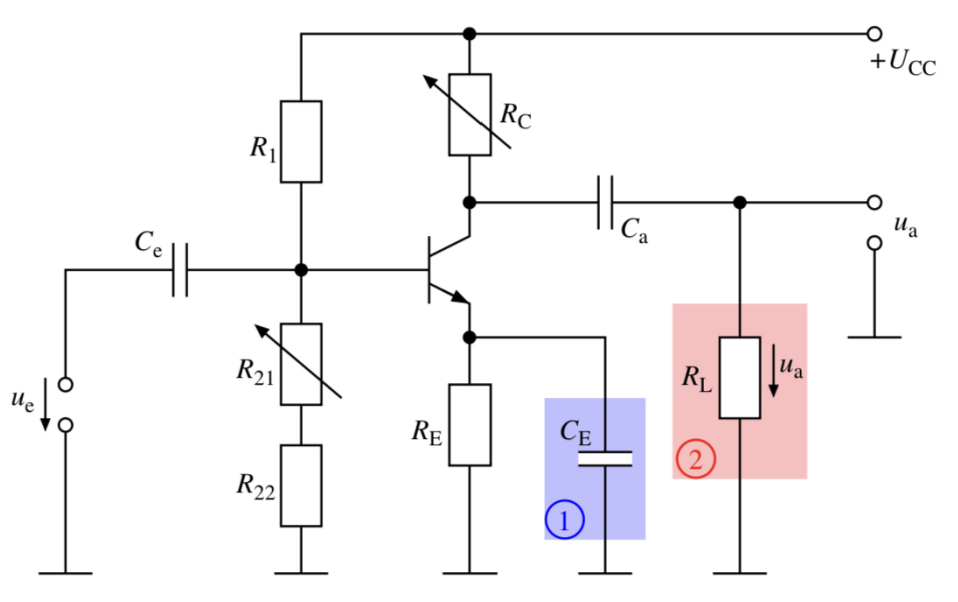
\includegraphics[width=0.8\textwidth]{bilder/Emitter circuit.png}
    \caption{emittercircuit:\\
    $R_1$ = 47 \si{\kilo\ohm}, $R_{22}$ = 100 \si{\ohm},$R_E$ = 10 \si{\kilo\ohm}, $C_e$ = 47 \si{\micro\farad},$C_a$ = 470 \si{\micro\farad}, $U_{CC}$ = 9 \si{\volt} 
    $R_{12}$: potentiometer for the operating point, $R_C$: potentiometer 0 - 10 \si{\kilo\ohm}, $u_e$: inputvoltage, $u_a$: outputvoltage
    }
    \label{im:Emcir}
\end{figure}

\subsection{Operating Point}
A bipolar transistor has a specific basevoltage range (the so called operating point) in which it behaves approximately linear. This operating point
is tuned by setting the resistance at the potentiometer $R_{12}$ \ref{im:Emcir}[see circuit diagram] to a point whereby the output amplitude $u_a$ is maximal and the signal is not distorted.
To tune the operating point, the load resistor $R_L$ was removed and a sinusoidal frequency of 5.5 \si{\kilo\hertz} was applied. 
$U_{\text{BE}}$, $U_{\text{CE}}$, $I_{\text{C}}$ where measured with varying $R_{\text{C}}$ for further evaluation.
\subsection{Amplification of the Emittercircuit}
To further examine the emitter circuit \ref{im:Emcir}[see circuit diagram] the amplitude ratio $u_a / u_e$ was measured for varying $R_{\text{C}}$ in different circuit configurations:\\
1. with capacitor $C{\text{E}}$ but without resistor $R_{\text{L}}$
2. without capacitor $C{\text{E}}$ and without resistor $R_{\text{L}}$
3. with capacitor $C{\text{E}}$ and resistor $R_{\text{L}}$
\subsection{Frequency Response}
In this experiment the input frequency was varied from 6 \si{\hertz} - 250 \si{\kilo\hertz} to measure the phaseshift and the amplidude ratio $u_a / u_e$. 
Here circuit \ref{im:Emcir} with an collector resistor of $R_{\text{C}}$ was used. In addition to that the oszilloscope was changed to x-y mode to observe lissajous curves.
\subsection{Characteristic Curve}
\begin{figure}[h]
    \centering
    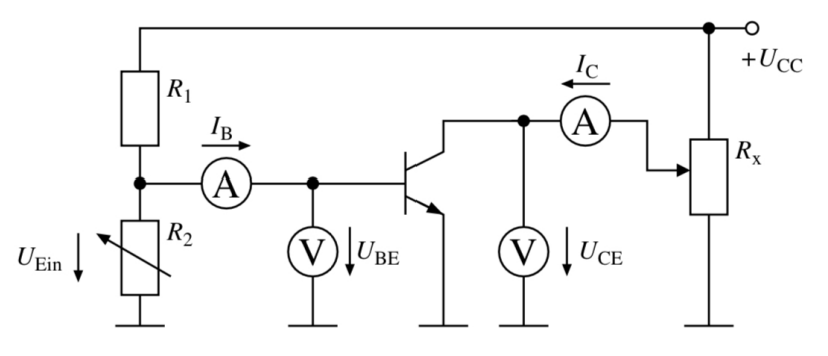
\includegraphics[width=0.8\textwidth]{bilder/characteristicCurve.png}
    \caption{characteristic curve \\
    $R_1$ = 1 \si{\kilo\ohm}, $R_2$ = 220 \si{\ohm}}
    \label{im:Charcurcir}
\end{figure}

To measure the characteristic curve of the transistor the circuit was change as shown in the circuit diagram \ref{im:Charcurcir}. 
First the entry curve $I_{\text{B}}=f(U_{\text{BE}})|_{U_{\text{CE}}}$ was taken by changing $U_{\text{BE}}$ from 0 to 670 \si{\milli\volt} and measuring $I_{\text{B}}$,
$U_{\text{BE}}$ and $U_{\text{CE}}$ with multimeters according to the schematic \ref{im:Charcurcir}. Therby $U_{\text{CE}}$ was dialed in to match the results from experiment 1 \ref{tab:operating point_measurement} with $R_{\text{C}}$ = 5 \si{\kilo\ohm}.
Afterwards the output characteristic curve $I_{\text{C}} = f(U_{\text{CE}})|_{U_{\text{BE}}}$ was recorded with a varying $U_{\text{CE}}$ from 1 - 10 \si{\volt} by measuring $I_{\text{C}}$, $U_{\text{BE}}$ and $U_{\text{CE}}$. This curve was measured in both directions to observe the effect of heat on the transistor.

\section{Evaluation and Results}
\subsection{Preliminary Considerations}

\subsubsection{Measuring of the characteristic Values}
The characteristic Values of a transistor are different for each operating point. Therefore the measurements have to be done with the Voltages already applied. While measuring, there is already a Voltage aplied. This could messs with the Multimeter leadiging to wrong measurements, if it assumes free floating ends. This also meand, that the resistance of the power supply and the resistor has to be taken into account, as is is essantialy a second path for energy to flow parallel. Lastly the test Voltage, which the multimeter uses to probe the resistance could be greater than the maximum of the small signal model, so that the multimeter measures outside the linear section.

\subsubsection{Transformation of y to h parameters}
The dependency of $i_1$, $i_2$, $u_1$ and $u_2$ can also be written in h parameter form as
\begin{align}
    \begin{pmatrix}
        u_1 \\
        i_1
    \end{pmatrix}
    = 
    \begin{pmatrix}
        r_{BE} & -S_r r_{BE} \\
        S r_{BE} & \frac{\frac{1}{r_{BE} \cdot r_{CE}} - S_r \cdot S}{r_{BE}}
    \end{pmatrix}
    \begin{pmatrix}
        i_1 \\
        u_2
    \end{pmatrix}
\end{align}


\subsection{Characteristic Curve (Assignment 7)}
As shown in table \ref{tab:operating point_measurement} some basevalues were recorded which were needed in following experiments. They seem to be in a reasonable range.

\begin{table}[H]
    \centering
    \begin{tabular}{c|c|c|c|c}
    
        $R_{\text{C}}$ in \si{\kilo\ohm}  & $U_{\text{BE}}$ in \si{\volt} & $U_{\text{CE}}$ in \si{\volt} & $I_{\text{C}}$ in \si{\milli\ampere} & $S$ in \si{1\per\ohm} \\ \hline
        1 & 0,57 & 7,86 & 0,58 & 0.025\\ 
        5 & 0,57 & 5,53 & 0,58 & 0.025\\ 
        10 & 0,57 & 3,22 & 0,58 & 0.025\\ 
    \end{tabular}
    \label{tab:operating point_measurement}
    \caption{Base values}
\end{table}

The characteristic input curve is plottet in figure \ref{fig:Eincur}. With the slope of the tangent one can calculate the base resistance $r_{\text{BE}}$ = 3.92 \si{\kilo\ohm} with equation \ref{eq:rbe}. 
The operating temperature $T$ = 272,2 \si{\kelvin} can be obtained by using the fitparameters from the exponetial fit and equation \ref{eq:Ib_T}. Although the operating temperature has the correct magnitude it should be at least 30 \si{\kelvin} higher.
With this operating temperature and equation \ref{eq:steep} the steepness $S$ can be calculated as shown in figure \ref{tab:operating point_measurement}.

\begin{figure}[h]
    \centering
    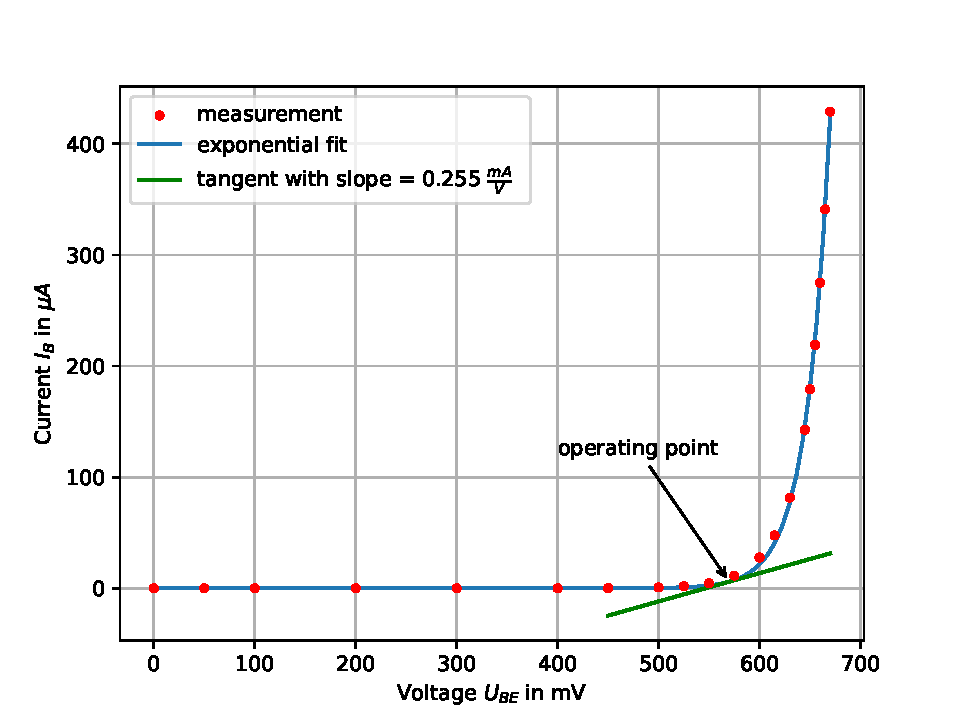
\includegraphics[width=0.8\textwidth]{plots/Eingangskennlinie.pdf}
    \caption{Characteristic curve from the input}
    \label{fig:Eincur}
\end{figure}

\begin{figure}[h]
    \centering
    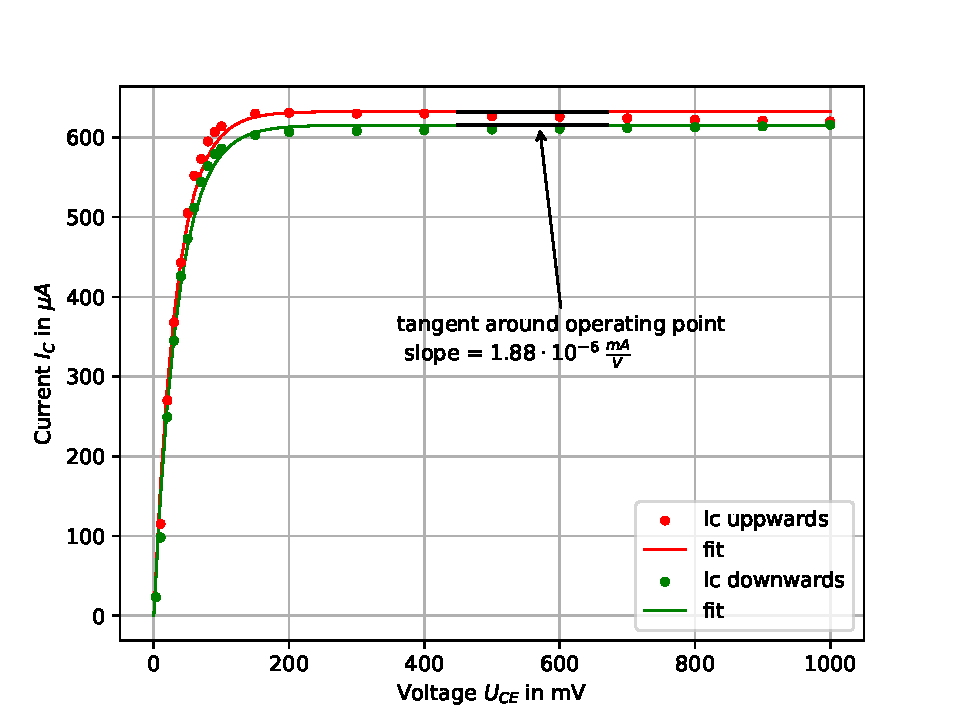
\includegraphics[width=0.8\textwidth]{plots/Ausgangskennlinie.pdf}
    \caption{Characteristic curve from the output}
    \label{fig:Outcur}
\end{figure}
The characteristic output curve is plottet in figure \ref{fig:Outcur}.




\bibliographystyle{plain}
\bibliography{literature}

\end{document}

